% PREAMBULA DOKUMENTA
\documentclass[a4paper]{article}
\usepackage[slovene]{babel}
\usepackage[utf8]{inputenc}
\usepackage[T1]{fontenc}
\usepackage{graphicx}
\usepackage {lmodern}
\usepackage{amsfonts}
\usepackage{amsmath}
\usepackage{amssymb}
\usepackage{tikz}
\usepackage{mathtools}
\usepackage{wrapfig}
\usepackage{commath}
\usepackage{listings}
\usepackage{color}


\definecolor{codegreen}{rgb}{0,0.6,0}
\definecolor{codegray}{rgb}{0.5,0.5,0.5}
\definecolor{codepurple}{rgb}{0.58,0,0.82}
\definecolor{backcolour}{rgb}{0.95,0.95,0.92}

\lstdefinestyle{mystyle}{
    backgroundcolor=\color{backcolour},   
    commentstyle=\color{codegreen},
    keywordstyle=\color{magenta},
    numberstyle=\tiny\color{codegray},
    stringstyle=\color{codepurple},
    basicstyle=\footnotesize,
    breakatwhitespace=false,         
    breaklines=true,                 
    captionpos=b,                    
    keepspaces=true,                 
    numbers=left,                    
    numbersep=5pt,                  
    showspaces=false,                
    showstringspaces=false,
    showtabs=false,                  
    tabsize=2
}

\lstset{style=mystyle}
 


\begin{document}
\thispagestyle{empty}

\begin{figure}[t]
\begin{center} 

\includegraphics[width=6cm]{fmf.png}\\[4cm]
\end{center}
\end{figure}

\begin{center}
\Huge\textbf{Katzova središčnost in Googlov PageRank}\\[0.5cm]
\large\textsc{Poročilo projekta pri predmetu Finančni praktikum}\\[4cm]
\end{center}

\begin{flushleft}

\end{flushleft}
\vspace{\fill}
\begin{flushright}
Anamari Oštarijaš, Tina Ražić
\end{flushright}

\begin{flushleft}
Ljubljana, december 2018
\end{flushleft}

\newpage
\tableofcontents

\newpage
\section{Opis projekta}
\hspace{4.8mm}Kompleksna omrežja lahko analiziramo z uporabo različnih kvantitetnih merjenj, imenujemo jih tudi mere središčnosti,  ki intuitivno zajamejo pomembnost določenih vozlišč. 
V projektu bova implementirali Googlov PageRank in Katzovo središčnost z uporabo potenčne metode. Na različnih grafih (tudi socialnih omrežjih) bova analizirali in primerjali, kako merjenji razvrstita vozlišča po pomembnosti. 

\section{Katzova središčnost}
\subsection{Matematično ozadje}


\hspace{4.8mm}Katzova središčnost izmeri vpliv igralca v omrežju tako, da upošteva direktne sosede igralca in vse druge igralce, ki so posredno povezani s tem igralcem preko njegovih direktnih sosedov. \\
Naj bo naše omrežje graf z $n$ vozlišči oziroma igralci. Vsaka povezava v grafu dobi utež $\alpha$ in z $\alpha^{d}$ izračunamo težo povezave vozlišča z drugim vozliščem, pri čemer je $d$ število povezav med njima. Naš graf predstavimo z matriko sosednosti A, torej element matrike $a_{ij}$ ima vrednost $1$, če je vozlišče $i$ povezano z vozliščem $j$, in $0$, če nista povezana. Potence matrike A nam povejo, če je vozlišče povezano s drugimi indirektnimi vozlišči preko sosedov. Na primer, če je v matriki $A^{3}$ element $a_{2,5}  = 1,$ pomeni, da sta vozlišče $2$ in vozlišče $5$ povezana s tremi povezavami preko sosedov prve stopnje in sosedov druge stopnje. \\
Označimo s $C_{Katz}(i)$ Katzovo središčnost vozlišča $i$. Potem lahko izračunamo središčnost na sledeči način:

$$C_{Katz}(i) = \sum_{k=1}^{\infty}\sum_{j=1}^{n}\alpha^{k}(A^{k})_{ij}.$$

Pri izbiri $\alpha$ moramo upoštevati zgornjo omejitev $$\alpha < \frac{1}{\abs{\lambda_{max}}}.$$
\subsection{Psevdokoda}

\section{Googlov PageRank}
\hspace{4.8mm}Nemogoče je definirati splošno mer pomembnosti, ki bi bila sprejemljiva za vse uporabnike iskalnika. Google uporablja pagerank za mero kakovosti spletnih strani. Temelji na predpostavki, da število linkov (povezav)  do in iz strani daje informacijo o pomembnosti strani. \\
Naj bodo vse spletne strani urejene s števili od $1$ do $n$ in naj bo $i$ neka spletna stran. Potem $O_i$ določa množico strani, s katerimi je i povezana, tako da $i$ vsebuje link do strani v množici $O_i$ (\textit{outlink}). Število outlinkov označimo z $N_i = \|O_i\|$. Množica \textit{inlinkov}, označena z $I_i$, je množica strani, ki imajo outlink do $i$ (strani v $I_i$ vsebujejo linke do $i$).
Splošno, več ko ima stran$i$ inlinkov, pomembnejša je. \\ Vseeno pa bi bilo s takim sistemom preprosto manipulirati (če bi nekdo želel, da njegovo spletno stran vidi čim več ljudi, bi ustvaril veliko število nepomembnih spletnih strani, ki bi vsebovale linke do njegove spletne strani). Da bi tako manipulacijo preprečili, definiramo rang vozlišča $i$ tako, da če ima visoko rangirana stran $j$ outlink do $i$, to doda pomembnosti $i$ na sledeč način: rang strani $i$ je utežena vsota rangov strani, ki imajo outlink do $i$. Obteženost  je taka, da je rang strani $j$ razdeljen enakomerno med njenimi outlinki. Z enačbo: $$r_i = \sum_{j \in I_1} \frac{r_j}{N_j}.$$ \\
Ta definicija je rekurzivna, zato pageranki ne morejo biti izračunani direktno. Uporabimo iteracijo. Najprej ugibamo začetni rangni vektor $r^0$. Potem iteriramo:
$$r_i^{(k+1)} = \sum_{j \in I_1} \frac{r_j^{(k)}}{N_j}$$ \\
Raje zapišimo problem z matrikami. Naj bo $Q$ kvadratna matrika dimenzije $n$. Definiramo:
\[
Q_{ij} = 
\left \{
	\begin{array}{ll}
		1/N_j  &, \mbox{če obstaja link od j do i }  \\
		0 &, \mbox{sicer} 
	\end{array}
\right. \]
\\
Torej ima vrstica $i$ neničelne elemente na mestih inlinkov $i$. Podobno ima stolpec $j$ neničelne elemente enake $N_j$ na mestih  outlinkov $j$, vsota vseh elementov v stolpcu je enaka $1$. Definicija je ekvivalentna skalarnem produktu vrstice $i$ in vektorja $r$, ki vsebuje range vseh strani.\\
Enačbo sedaj lahko zapišemo v matrični obliki:
$$ \lambda r = Qr,     \qquad \lambda = 1,$$
Tako dobimo, da je $r$ lastni vektor matrike $Q$ z lastno vrednostjo $\lambda = 1$. Sedaj preprosto vidimo, da je iteracija ekvivalentna
$$r^{(k+1)} = Qr^{(k)},\qquad  k=0,1,… ,$$
kar je potenčna metoda za izračun lastnega vektorja.\\
\\ \textbf{Problem}: Ni jasno, da je pagerank dobro definiran, saj ne vemo ali obstaja lastna vrednost enaka 1. Pomagamo si s teorijo Markovske verige.\\
\\Obstaja interpretacija pageranka z naključnimi sprehodi. Predpostavimo, da uporabnik na spletni strani izbere naslednjo stran  med outlinki z enako verjetnostjo. Markovska veriga je slučajni proces v katerem je naslednje stanje določeno le s trenutnim stanjem, proces nima spomina. Prehodna matrika Markovske verige je $Q^T$.\\
Slučajni uporabnik nikoli ne sme obtičati. Z drugimi besedami, naš model slučajnega sprehoda ne sme imeti strani brez outlinkov (taka stran bi imela stolpec iz ničel v $Q$). Torej je model prilagojen tako, da so ničelni stolpci nadomeščeni s konstantnimi vrednostmi na vseh mestih. To pomeni, da je enaka verjetnost, da pridemo na katero koli drugo spletno stran. \\ 
\\Definiramo vektorje: \\
\[
d_j = 
\left \{
	\begin{array}{ll}
		1  &, \mbox{če} N_j = 0 \\
		0 &, \mbox{sicer} 
	\end{array}
\right. \]
za $j = 1, .., n$ in
$$e = [1 … 1] ^T \in \mathbb{R}^n.$$
Prilagojena matrika je definirana s $ P = Q + \frac{1}{n}ed^T$. 
S to prilagoditvijo je matrika $P$ desna stohastična matrika; vsi elementi so nenegativni in elementi vsakega stolpca se seštejejo v 1. \\
\\Desna stohastična matrika $P$ zadošča 
$$e^TP = e^T$$. \\
Želimo definirati pagerank vektor kot enoličen lastni vektor matrike $P$ z lastno vrednostjo $1$:
$$Pr=r$$. \\
Lastni vektor prehodne matrike je stacionarna verjetnostna porazdelitev Markovske verige. Element na mestu $i$ ($r_i$) je verjetnost, da po velikem številu korakov slučajni uporabnik pristane na strani $i$. Za zagotovitev enoličnosti mora biti matrika ireducibilna (slučajni uporabnik se lahko v nekem delu grafa zagozdi, v tem primeru ima matrika več lastnih vrednosti enakih $1$). \\ Edinstvenost največje lastne vrednosti ireducibilne, pozitivne, desne stohastične matrike je zagotovljena s \textit{Perron-Frobeniusovim izrekom}, največja singularna vrednost bo enaka $1$, pripadajoč slastni vektor je pozitiven in je edini lastni vektor, ki je nenegativen. \\
\\Zaradi velikosti spleta je matrika linkov $P$ reducibilna, torej pagerank lastni vektor ni dobro definiran. Da si zagotovimo ireducibilnost, umetno dodamo linke iz vsake spletne strani do vseh drugih. To lahko storimo, če vzamemo konveksno kombinacijo $P$ in matrike ranga 1:
$$A=\alpha P + (1-\alpha)\frac{1}{n}ee^T,$$
za nek $\alpha$, ki zadošča $0 \leq \alpha \leq 1$. Matrika $A$ je desna stohastična. Razlaga naključnega sprehoda dodatnega rang-1 izraza je, da bo uporabnik na vsakem časovnem koraku skočil na naključno stran z verjetnostjo $1- \alpha$.
Za konvergenco numeričnega algoritma za lastno vrednost je pomembno, da vemo, kako so s prilagoditvijo ranga-1 spremenjene lastne vrednosti.\\
\\ \textbf{Izrek:} \textit{Naj bodo lastne vrednosti desne stohastične matrike $P$ enake ${1, \lambda_2, \lambda_3, … , \lambda_n}$. Potem so lastne vrednosti $A=\alpha P + (1- \alpha) \frac{1}{n}ee^T$ enake ${1, \alpha \lambda_2, \alpha \lambda_3, … , \alpha \lambda_n}$.}\\
\\
Ta izrek nam pove, da tudi če ima $P$ več lastnih vrednosti enakih 1, kar je po navadi res, bo druga največja lastna vrednost matrike $A$ enaka $\alpha$. \\
Namesto prilagoditve lahko definiramo:
$$A = \alpha P + (1- \alpha)ve^T,$$
Kjer je $v$ nenegativen vektor z normo 1, ki je lahko izbran tako, da je iskanje pristransko do strani določene vrste. Zato ga včasih imenujemo \textit{personaliziran vektor}. Uporaben je tudi v izogib manipulacijam proti t.i.\textit{link farms}. 

\subsection{Potenčna metoda}
Želimo rešiti problem lastne vrednosti:
$$Ar = r,$$
Kjer je $r$ nomaliziran $\|r\|_1=1$. Iskani lastni vektor označimo s $t_1$. \\
Prepostavimo, da imamo dan začetni približek $r{(0)}$. \\
\\
\textbf{Algoritem:} \\
\begin{center} za k = 1, 2, … do konvergence
	$$q^{(k)} = Ar{(k-1)}$$ 
	$$r^{(k)} = q^{(k)}/ \|q^{(k)}\|_1$$ \\
\end{center}
Konvergenca je odvisna od porazdelitve lastnih vrednosti. Če je druga največja lastna vrednost blizu 1, bo iteracija zelo počasna. To na srečo ne velja za Google matriko. Vektor normaliziramo, da ne bi z iteracijami postali preveliki ali premajhni, posledično nereprezentativni s števili s plavajočo vejico. To v resnici ni potrebno, saj se v primeru desnih stohastičnih matrik temu izognemo.

\subsection{Algoritem za Googlov PageRank}
\begin{lstlisting}[language=Python]
def Qmatrix(matrika):
    '''za dano matriko sosednosti grafa vrne desno stohasticno matriko Q, kjer so nekateri stolpci se vedno nicelni'''
    sums = np.sum(matrix, axis=0)       #tabela vsot stolpcev matrike
    return np.nan_to_num(matrix/sums)   #vsak stolpec matrike delimo z njegovo vsoto, ce je vsota 0, vrne 0 namesto nan

def dvector(matrika):
    '''za dano matriko sosednosti vrne transponiran vektor d, kjer d[j] = 1 ; ce #(outlinkov od j) = 0 in d[j] = 0 ; sicer'''
    Q = Qmatrix(matrix)             #izracunamo matriko Q
    sums = np.sum(matrix, axis=0)   #tabela vsot stolpcev matrike
    d_bool = (sums == 0)            #bool tabela, True ce je vsota stolpca enaka 0 in False sicer
    d = d_bool*1                    #False v 0 in True v 1
    return d

def evector(n):
    '''vrne vektor v iz samih enk velikosti n, kjer n = st. stolpcev v matriki'''
    return np.ones((n,1))    

def Pmatrix(matrix):
    '''vrne desno stohasticno matriko P'''
    n = matrix.shape[1]
    Q = Qmatrix(matrix)
    e = evector(n)
    d = dvector(matrix)
    return Q + 1/n*e.dot(d)

def Amatrix(matrix, alpha):
    '''vrne ireducibilno desno stohasticno matriko A, kjer je 0 <= alpha <= 1'''
    n = matrix.shape[1]
    e = evector(n)
    P = Pmatrix(matrix)
    return alpha*P + (1-alpha)*1/n*e.dot(e.transpose())

def pagerank2(matrix, max_num_of_steps, tolerance, alpha):
    '''vrne pagerank vektor matrike sosednosti grafa, 0<=alpha<=1'''
    start = timer()
    A = Amatrix(matrix, alpha)           #desno stohasticna matrika dane matrike
    r = A[:,0]  			    #ugibanje pagerank vektorja s prvim stolpcem matrike Q
    diff = 1000
    k = 0
    while diff > tolerance and k < max_num_of_steps:
        r, q = A.dot(r), r                             #potencna metoda
        #r = q/np.linalg.norm(q, ord=1)    #ni potrebno pri Google matriki
        diff = np.linalg.norm(q-r, ord=1)   #razlika med prejsnjim in novim vekorjem r
        k+=1
    print('proces koncan po {} iteracijah'.format(k))
    end = timer()
    print('trajanje procesa: {} sekund'.format(end-start))  
    return r


\end{lstlisting}

\subsection{Analiza algoritma}
\hspace{4.8mm}Analizirali sva učinkovitost algoritma na podlagi večih parametrov. Najbolj naju je zanimalo, kako izbira parametera $\alpha$, toleranca in število korakov vplivajo na hitrost algoritma in natančnost rezultata. \\
Uporabljali sva \textit{Facebook graf}, ki vsebuje $4039$ vozlišč in $88234$ povezav.
\begin{figure}[h]
\begin{center} 
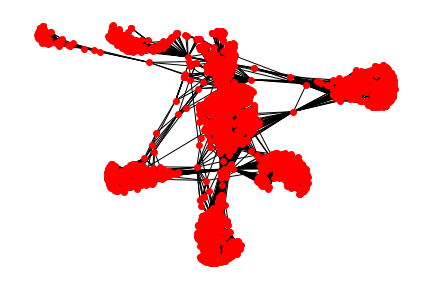
\includegraphics[width=6cm]{Facebook_graph.png}
\end{center}
\end{figure}

\subsubsection{Izbira parametra $\alpha$} 
\hspace{4.8mm}Vemo, da večji ko je $\alpha$, več podatkov o omrežju izgubimo. Torej želimo, da je ta parameter čim večji. \\
Poglejmo najprej kako velikost vpliva na čas izračuna pagerank vektorja. 

\begin{lstlisting}[language=Python]
M_fb = nx.adjacency_matrix(G_fb)
r_1 = pagerank2(M_fb,10000000,0.0000001, 0.98)
print(r_1)
----------------------------------------------------------------
proces koncan po 575 iteracijah
trajanje procesa: 11.7118154744594 sekund
[[  4.79508113e-03]
 [  2.17910466e-04]
 [  1.52316417e-04]
 ..., 
 [  6.77736016e-05]
 [  1.25649865e-04]
 [  2.72346363e-04]]
\end{lstlisting}

Izračun je bil končan po $575$ iteracijah in $11,71$ sekundah.

\begin{lstlisting}[language=Python]
r_2 = pagerank2(M_fb,10000000,0.0000001, 0.999)
print(r_2)
----------------------------------------------------------------
proces koncan po 4719 iteracijah
trajanje procesa: 61.73710875091092 sekund
[[  2.37207123e-03]
 [  1.15387662e-04]
 [  6.99886732e-05]
 ..., 
 [  2.37766591e-05]
 [  4.70770334e-05]
 [  1.04002744e-04]]
\end{lstlisting}
S povečanjem $\alpha$ smo povročili, da se je čas izračuna povečal na $61,74$ sekund, torej za več kot $5$ kratnik prejšnjega. 

\begin{lstlisting}[language=Python]
r_4 = pagerank2(M_fb,10000000,0.0000001, 0.9999)
print(r_4)
----------------------------------------------------------------
proces koncan po 8104 iteracijah
trajanje procesa: 105.30294071864228 sekund
[[  1.99799361e-03]
 [  9.77897213e-05]
 [  5.77554403e-05]
 ..., 
 [  1.28541957e-05]
 [  2.56615989e-05]
 [  5.75079410e-05]]
\end{lstlisting}
\newpage
Večji ko je $\alpha$, več iteracij potrebujemo, da pridemo do željene tolerance. \\
Razlika med $r_1$ in $r_2$ v drugi normi je $0,00717920758147$, med $r_2$ in $r_4$ pa $0,00371765512728$, torej lahko z višjim $\alpha$ pričakujemo bolj natančne rezultate.  
\begin{figure}[h]
\begin{center} 
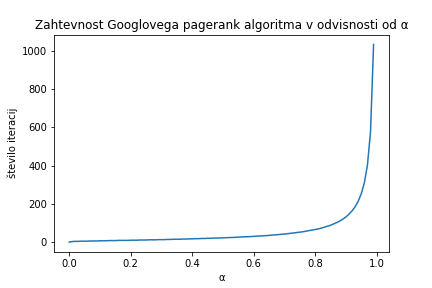
\includegraphics[width=10cm]{Pagerank_alpha.png}
\end{center}
\end{figure}
\begin{figure}[h]
\begin{center} 
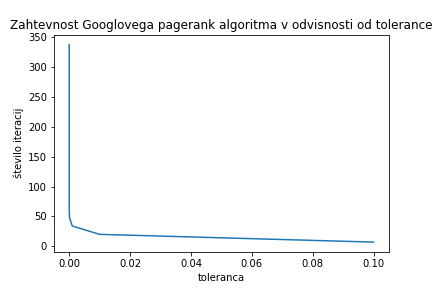
\includegraphics[width=10cm]{Pagerank_tolerance.png}
\end{center}
\end{figure}

\section{Primerjava algoritmov}
\end{document}
